% ============================================================
%  INTRODUCTION: Meera's dollar problem        (Member 1)
%  15 Nov 2026: text replaced with Member 1's shorter version
%  (Member1_Changes.md). "Questions this chapter answers" box removed.
% ============================================================
\section*{Introduction: Meera's dollar problem}
\addcontentsline{toc}{section}{Introduction}

In October 2026, Meera, a Class 12 student in Chennai, won a place at a college in the United States. Its first-year fees were US\$40,000, the same as a year earlier. Yet in rupees they now cost about ₹2.5 lakh more.\sidenote{The fees are hypothetical. The rates are real closing rates: ₹88.67 per US\$ on 13 October 2025\cite{bs2025b} and ₹95.05 on 15 October 2026.\cite{hdfc2026} 40,000 × 6.38 = ₹2,55,200.} The college hadn't raised its price. The price of the dollar had gone up.

Her uncle Ravi, an electrician in Dubai, saw the other side. The money he sends his parents in Thanjavur every month now arrives as more rupees. One price, two opposite outcomes (Figure~\ref{fig:comic-intro}). This chapter explains what that price is, who sets it and why it keeps moving.

\begin{figure}[H]
  \centering
  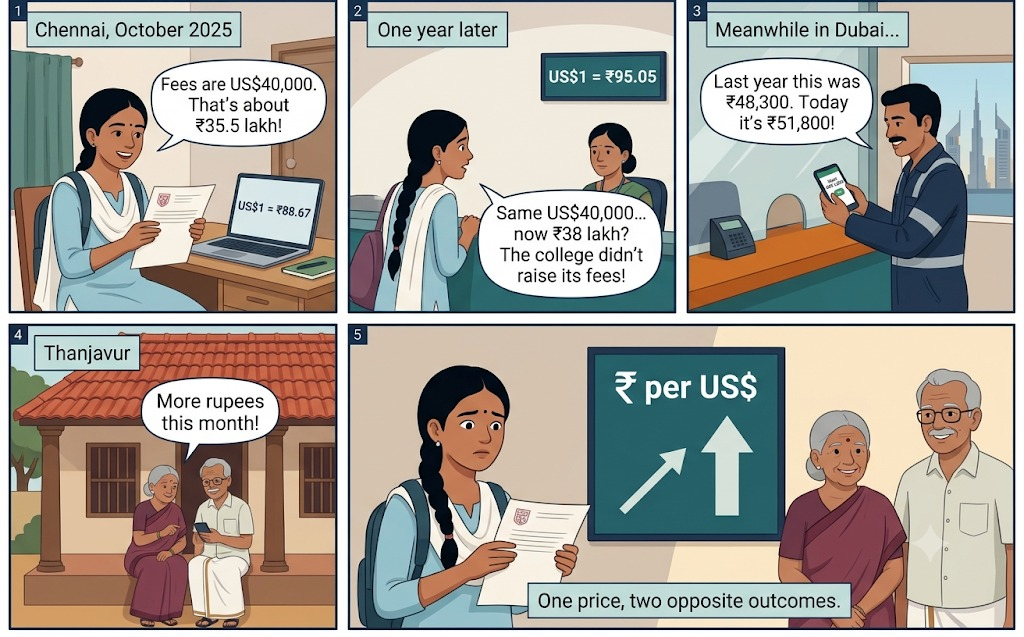
\includegraphics[width=0.85\linewidth]{images/comic2.png}
  \caption{One price, two opposite outcomes.}
  \label{fig:comic-intro}
\end{figure}
